\documentclass[11pt]{article}

%\usepackage{amsmath, amssymb, fullpage, amsthm, array, algorithm2e,graphicx}
\usepackage{graphicx, amsmath}
\usepackage{url}
\RequirePackage{natbib}
\usepackage[colorlinks=true, citecolor=blue, linkcolor=blue]{hyperref}

\graphicspath{{images/}}

\setlength{\oddsidemargin}{0in}
\setlength{\evensidemargin}{0in}
\setlength{\textwidth}{6.5in}
\setlength{\topmargin}{-0.3in}
\setlength{\textheight}{8.8in}


%\setlength{\evensidemargin}{0.25 in}
%\setlength{\textwidth}{6.2 in}           % allow for a little sloppiness (6.3)
%\setlength{\topmargin}{-.30 in}           % top margin to header (was -.35)
%\setlength{\textheight}{8.8 in} 


\title{Designing Turk Experiments for Visual Statistical Inference}
\author{Mahbubul Majumder, Heike Hofmann, Dianne Cook\\
        Department of Statistics, Iowa State University}


\begin{document}

\tableofcontents

\maketitle


\begin {abstract} 

Human observers are needed to evaluate lineups that are used to test the significance of findings using statistical graphics. One good option is to recruit people from online workplace like Amazon Mechanical Turk (MTurk). It provides features to create online task that allow people to evaluate lineups and get paid. MTurk is designed for simple and easy tasks. The technical design of the underlying experiment for lineup evaluation may be complex and the tools available to design this from MTurk is just too simple. In this paper we present the design of MTurk experiments for lineup evaluation, provide an alternative way to conduct the survey on lineups by developing a separate web application and getting turk worker do their job from that web site. The web site is now hosted on the Iowa State University public domain and has been in use for multiple experiments \citep{majumder:turk}. It provides multiple features that make it convenient to get lineups evaluated by online observers and obtain data in a secure way.

{\bf Keywords: \sf statistical graphics, lineup, Amazon Mechanical Turk, visual inference, visualization, Crowdsourcing, Human Intelligence.}

\end {abstract}


\section{Introduction} 

There have been some advancements in visual statistical inference since the concept was first introduced by \cite{buja:2009}. They  proposed lineup protocol that allows testing the significance of findings using statistical graphics. In visual statistical inference the test statistics is a plot of the observed data. This plot is placed randomly in a layout of plots called lineup. The rest of the plots, called null plots, in the lineups are generated using the data simulated from the model specified by the null hypothesis. A human observer is asked to evaluate the lineup. If the observer can detect the actual plot in the lineup, the null hypothesis is rejected. 

A lineup is shown in Figure~\ref{fig:lineup_turk} where the observed scatterplot is displayed with a least square line overlaid. Can you find which of these plots show the steepest slope? The null plots are generated based on the hypothesis that the slope is zero. If the observed scatterplot is detected, it indicates that observed plot is different from the null plots and hence provides evidence against the null hypothesis.

\begin{figure}[htbp] 
   \centering
   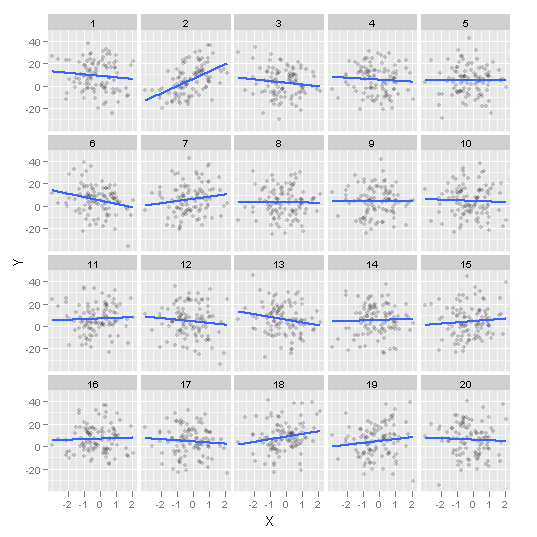
\includegraphics[width=6.5in]{plot_turk2_100_450_12_3.png} 
   \caption{A lineup of 20 scatter plots with least square line overlaid. Which of these plots shows the steepest slope? Answer to this question can be found at the end of conclusion.}
   \label{fig:lineup_turk}
\end{figure}


\cite{majumder:2013}  further developed visual statistical inference by refining the terminologies, presenting the ways to compute $p$-values associated with the visual test and providing the methods of obtaining the power of the test. It is revealed that the power of visual test  can be as good as that of the best available conventional test and in some scenarios even better. This work establishes the validity of lineup protocol to be used as a tool for statistical testing. In the situations where no conventional test exists, visual inference can be the only inferential procedure that does not compromise a lot on power because of its non-parametric nature and few assumptions. 

These developments open up a new area of statistical research where lineups need to be evaluated by human observer. For small scale or day to day research it is possible to have people around to get the lineups evaluated. But sometimes it is needed to have many observers to evaluate lineups. For example, to assess the power of the visual test for different visual test statistics \cite{heike:2012} recruited human observers to evaluate lineups.  \cite{niladri:2012} used lineup protocol in practical applications. Other reasons to evaluate lineups may be to present the results of the conventional test with visual tools such as lineup.  



%The effect of different graphical design while selecting visual test statistic is studied by Heike \cite{heike:2012}.

The power of visual test can be obtained theoretically under some assumptions on individual behavior which was evident from experimental studies \citep{majumder:2013}. In general it is hard to obtain explicitly with a mathematical formula since it is very much dependent on human observation. One approach to estimate the power is to recruit observers to evaluate lineups generated with some known effect sizes. The proportion of correct evaluation can be used as an estimate of the power for that effect size. Individual differences in the abilities of correct evaluations of lineup were observed. Thus it is desirable to get observers as diverse as possible.  

%without being much concerned about the observers' formal training about statistical graphics.

This poses a new challenge to researcher to recruit people from a diverse pool of population. Cost, time, data qualities and convenience are some of the issues that need to be dealt with. Fortunately, we can use the services of Amazon Mechanical Turk web site for this which is discussed in the following section.

\subsection{Amazon Mechanical Turk (MTurk)}

\cite{turk} Mechanical Turk  or MTurk is an online work place where people from around the world can perform tasks and get paid. Usually tasks are very simple and no specialized training is necessary. Being a human is the main requirement. Tasks are designed for anyone to do but some tasks may require that workers satisfy some skill level depending on the recruiters' need. The tasks are designed to be done in a very short time. Humans are still better than computers in performing these types of tasks. The the amount of money paid for each task is very small as well. Figure~\ref{fig:amazon_task} shows an MTurk task where an observer is asked to select an option based on a picture. 


\begin{figure}[htbp] 
   \centering
   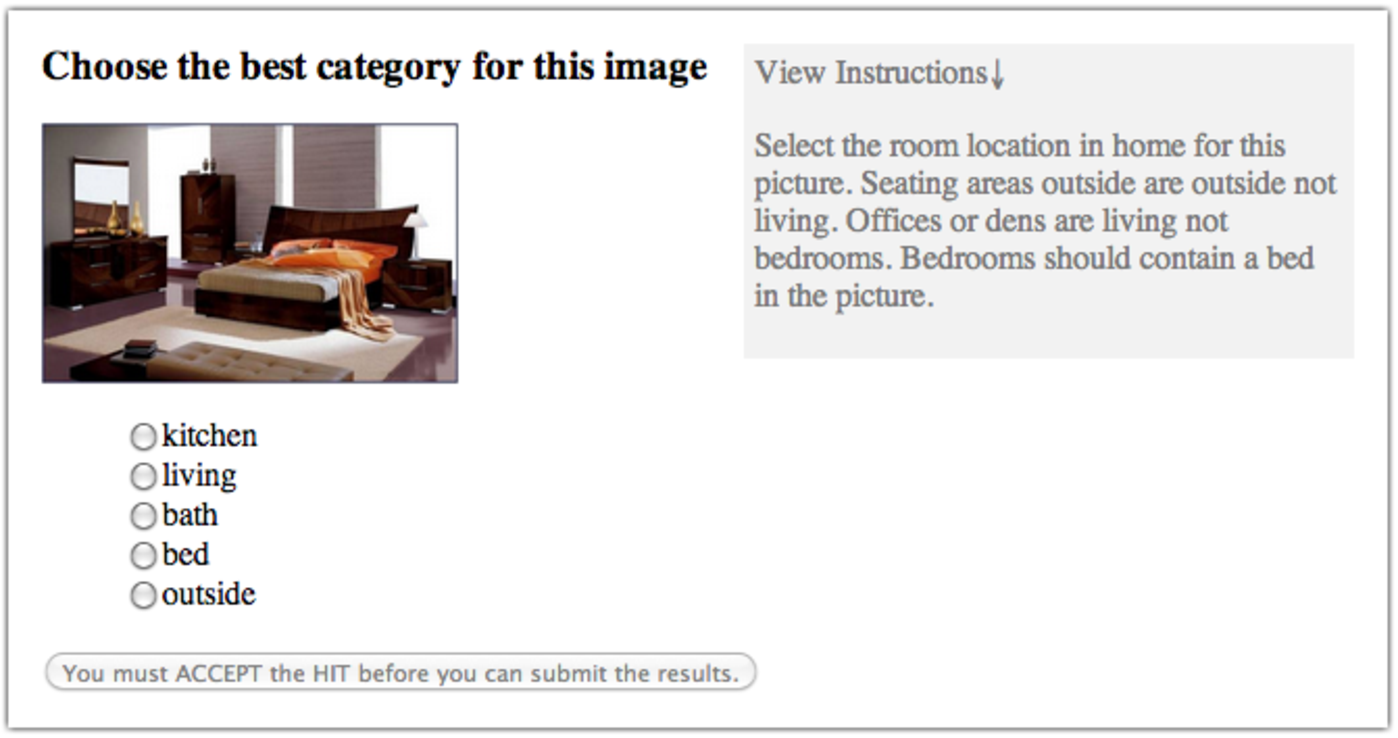
\includegraphics[width=5in]{amazon_task.pdf} 
   \caption{An example of amazon mechanical turk task. Tasks are usually very simple and designed for human evaluations. With each task, simple instructions are given for workers to follow. The workers first accept the task before submitting their response.}
   \label{fig:amazon_task}
\end{figure}

It is very cheap and reliable to recruit people from MTurk and the results can be obtained very fast. It allows distributing works to the thousands of workers around the world. The another benefit is that a very diverse pool of subjects can be recruited which is otherwise very hard to obtain for a study. The researchers can easily filter the workers based on their experimental design, such as recruiting people only from a specific geographical location or a group of people who satisfy certain criteria etc. The recruiter can decide who they pay or not. Workers have to satisfy the task requirement to ensure payment. But at the end it is the recruiter who has the final say. Usually recruiters pay promptly after the task has been done properly and thats why MTurk is very popular among the online job seeker.  

%It is also getting very popular among the researchers who perform human subject experiment. 

Because of its convenience it is getting popular for scientific research study as well. In comparison with a lab study \cite{suri:2010} performed the same study using MTurk and demonstrated that their study results are as good as the lab study results even though MTurk study required less time and cost while provided more convenience. \cite{majumder:2013} recruited people from MTurk for their simulation study in estimating the power of visual statistical inference. They have done numerous pilot studies in lab before doing actual MTurk study and found similar results. \cite{mason:2012} explains various features of MTurk and describes how it can be used as part of human behavioral study.

The simplicity of the MTurk task is the main factor for its popularity. Figure \ref{fig:amazon_task} shows how simple an MTurk task could be. It is possible to get a lineup evaluated by creating such a simple task. We just need to replace the picture in Figure \ref{fig:amazon_task} with the lineup in Figure \ref{fig:lineup_turk} and change the answering options. But some times we may need more than one lineups to be evaluated by an observer. We may need to show a random sample of lineups from a pool of many lineups automatically. The questions the observer would answer while examining the lineup can be different based on different lineups. Moreover, It is convenient if the lineup is clickable so that selection of plot can be made by the mouse click. To create an MTurk task that has all these flexibilities, a web application needs to be created. The following section discusses how the system would work.



%Amazon Mechanical Turk web site \cite{turk} is a very good resource for recruiting reliable survey participants for visual experiments. This is the place where people come to work online and get paid. The web site is very convenient and reliable to collect simple experiment data. But to design a complex experiment like what we need using their web interface is a pain and often a very time consuming work. So, to run the turk experiment we felt the necessity for a well customized web site where the lineups presented to the observers could be easily controlled according to the experimental design. The work flow design of such a mechanism is shown in figure \ref{fig:turk_work_flow}. The plan is to forward turk workers to a well customized web site while payment could be processed from turk web site. This facilitates getting data directly in a local server.

%Figure \ref{fig:amazon_task} displays an example of such a task taken from their web site. In this task a worker just has to select from a pool of options and submit the task. The instructions are usually accompany the task and they are very simple and easy to follow. 

\subsection{Getting Turk Workforce}

Once a web application is created, there are two options to run it; one is to run it inside MTurk system using their API and the other is to develop a new web site separate from MTurk. For additional control we picked the second option and planned to separate this application from MTurk system and designed our own web site to run the application. It enables us to display the lineups to the observers with a lot of flexibilities. As an added benefit the data can be directly saved in a local database server instead of getting it from MTurk. 

Figure \ref{fig:turk_work_flow} shows how the plan works. First an MTurk task is created for the workers to review and decide whether they want to do the task based on the parameters like payment amount, estimated time the task may take to finish and how hard the task seems to be etc. Workers are informed that the task has to be done outside the MTurk system from another web site. Once the workers accept the task they are redirected to our web site where multiple lineups are shown for evaluations. After the required number of evaluations has been received, a code is generated which the workers need to submit back in MTurk system to complete the task. The code is matched with the code in our database to process payment through MTurk system.

\begin{figure}[htbp]
   \centering
       \scalebox{.4}{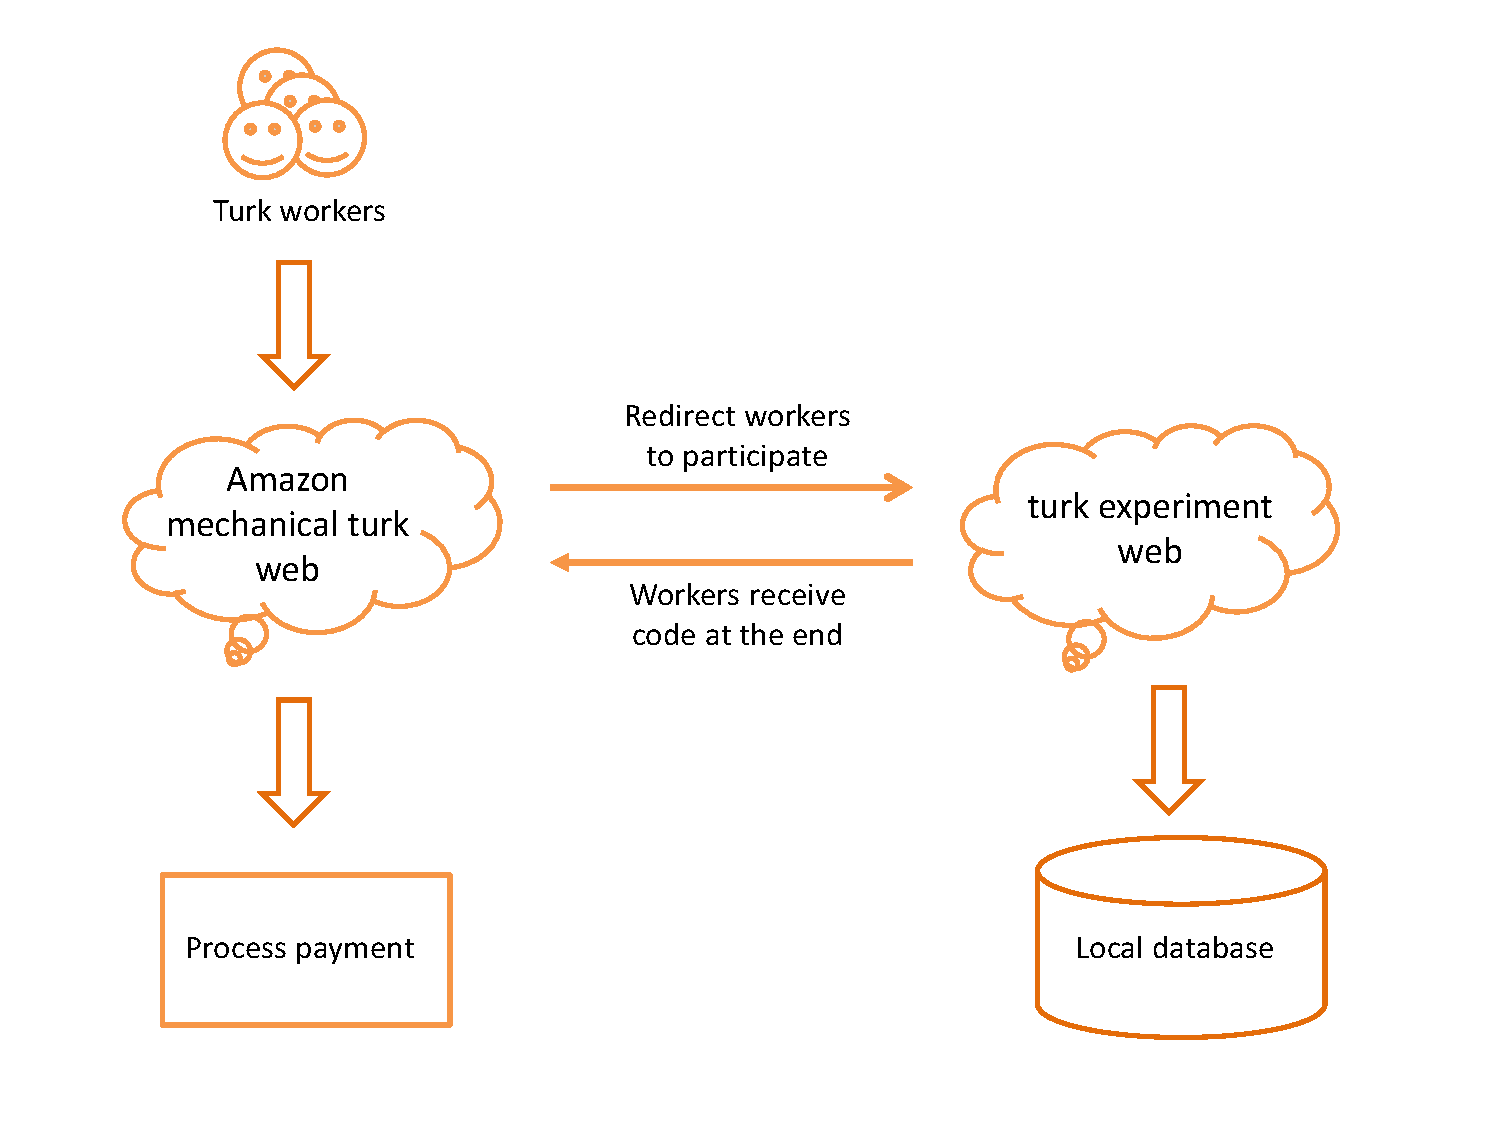
\includegraphics{turk_work_flow.pdf}}
       \caption{Amazon Mechanical Turk workflow shows how data are collected through turk experiment web and payment is processed through MTurk system.}
       \label{fig:turk_work_flow}
\end{figure}

MTurk provides workers who usually do the simple tasks available for them. Thus, for lineups to be evaluated a simple task needs to be created through MTurk. This may be a challenge for the researchers who want to make statistical decisions based on lineups or need to study the power of visual tests. They need a system that can provide an easy solution to this challenge while giving them flexibilities how they want to present the lineups. This paper provides a complete solution to this. It is organized the way a researcher may work with the experiments related to lineups and like to get feedback data from the observer. Section \ref{sec:turk_exp} presents the detailed description of an experiment with lineups and things to consider while creating a turk task. Section \ref{sec:web_application} presents the design of an web application to get lineups evaluated with additional flexibilities and options that may not be possible through MTurk. Section \ref{sec:turk_task} describes how to create an MTurk task, mange workers and process payments. Finally Section \ref{sec:turk_data} presents some data obtained from various experiments done through the web application and discusses about the quality of the data.


\section{Experiment Design} \label{sec:turk_exp}

If a lineup is created from the actual observed data, the web application presented in Section \ref{sec:web_application} can be used to get it evaluated. In that case we do not need to design a simulation experiment. This section will be useful when a simulation experiment is needed to examine different visual test statistics and compare the power \citep{majumder:2013}. To examine the effectiveness of certain plots in displaying the data one may want to design an experiment with lineup \citep{heike:2012}. In any cases, the two major considerations are the choice of parameters to simulate lineups and number of people needed to evaluate a lineup.

\subsection{Selecting Parameter to Simulate Lineup} \label{sec:parameter_selection} In any experimental design we need to have some control. For a simulation experiment with lineup, this refers to the parameters related to a lineup. This depends on what the purpose of the experiment is. For example, to compare the power of a parametric test one may fix the parameter specified by alternative hypothesis and generate data from that model. This data can be considered as the observed data. A lineup can be created by placing this observed data plot in a layout where rest of the data plots come from the model specified by the null model \citep{majumder:2013}. 

In addition to the hypothesized parameter of interest, other parameters that may need to be fixed include sample sizes, variability in the data, error structure etc. These parameters produce the effect sizes and are responsible for any detectable signal in the lineup. Thus for a simulation study a range of effects sizes need to be considered. It is a little bit tricky to decide what exact effect sizes are appropriate. For example in \cite{majumder:2013} the parameters were chosen so that they produce a smoother power curve of a conventional test. But in general this depends on what the researchers may want to test and control in an experimental study.

%The very first consideration is the sample size. Other parameters depends on the model of interest. For example we have fixed the parameters in our first Amazon Mechanical Turk experiment as shown in table \ref{tbl:experiment_params}.

\subsection{Procedure to Simulate Data Plot} \label{sec:simulate_plot} In the simulation study the very first step is to generate a random sample of data from the model of interest with pre-specified parameters. We call this data set observed data. Every time we do that we get a new set of observed data which may produce an estimated parameter very different than the actual parameter specified to generate the data. But it is important to have an observed data closely representing the parameters chosen since other null plots will be compared to this data plot in a lineup. One solution to this is to take some replications of lineups for the same effect size. 

While the effect of the natural variability of the observed data set can be controlled by taking the replication of few samples, it is desirable to study whether we can reduce this variability further to some extent. For this we pick the example of a simple linear regression model and examines how the data plot can be generated that best represents the specified parameter.  Consider a linear regression model 
\begin{equation} \label{eqn:turk_model} 
Y_i = \beta_0 + \beta X  + \epsilon_i 
\end{equation}
where $\epsilon_i \stackrel{iid}{ \sim } N(0,\sigma^2)$, $i=1,2, .., n$. The covariate $X$ can be continuous or discrete. As discussed in Section \ref{sec:parameter_selection} we specify the parameters sample size $n$=300, regression slope $\beta$=3 and error standard deviation $\sigma$=12 to simulate observed data.

To make sure that the observed data set truly represents the Model \eqref{eqn:turk_model} we suggest three approaches. One is Kolmogorov test statistic approach and the other two approaches are quantiles of $p$-values and closeness of estimated parameters to the true parameters. To illustrate the three approaches we used Model \eqref{eqn:turk_model} as an example but the idea can be extended to any situation. The three approaches are discussed below. \\

{\bf Kolmogorov test statistic approach:} In this approach we simulate 1000 data sets from Model \eqref{eqn:turk_model}  and obtain Kolmogorov test statistic for each set of data as below. $$D_n=\sup_x |F_n(x)-F(x)|$$ where $F_n(x)=\frac1n \sum_{i=1}^n I_{X_i\le x}$ be the empirical distribution function of fitted residuals, $I_{X_i\le x}$ be the indicator function equal to 1 if $X_i\le x$ and equal to 0 otherwise and $F(x)$ be the cumulative function of normal with mean zero(0) and variance $\sigma^2$. We keep the data set that has minimum value for Kolmogorov test statistic since for this data set $F_n(x)$ should be the closest to the desired normal model.  \\

{\bf Quantiles of $p$-value approach:} For a simulated observed data set we can obtain the $p$-value associated with testing $H_0: \beta=0$. The distribution of $p$-value is uniform under null hypothesis but under alternative it has a right skewed distribution. Figure~\ref{fig:dist_pvalue} shows the distribution  of $p$-values for sample size $n$=300, regression slope $\beta$=3 and error standard deviation $\sigma$=12. If we generate a data set randomly there is a 21\% chance that the data will show a $p$-value of 0.25 or more even though we generated data set with non-zero $\beta=3$. We need to make sure that the simulated data does not come from this extreme end. Additionally, we want some replications so that this extreme effect can be controlled at some level. For this example we intend to pick three replications.


\begin{figure}[hbtp]
   \centering
       \scalebox{.6}{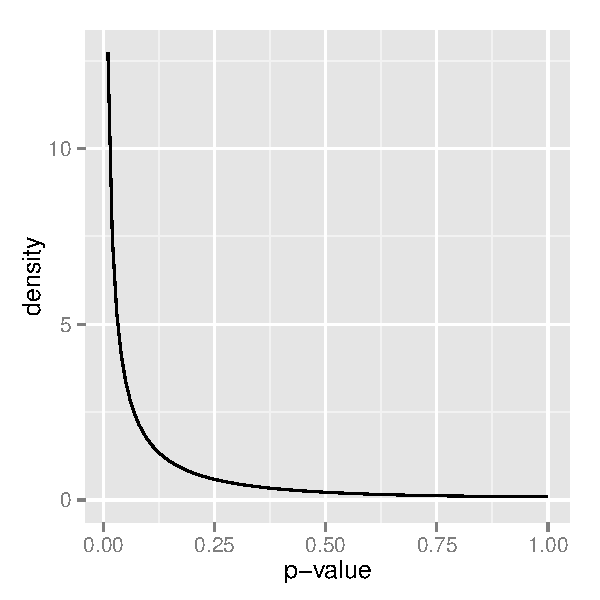
\includegraphics{dist_pvalue.pdf}}
       \caption{Distribution of $p$-values under alternative hypothesis ($H_1: \beta$=3) for sample size $n$=300 and error standard deviation $\sigma$=12.}
       \label{fig:dist_pvalue}
\end{figure}

In this approach we generate 1000 data sets from the model of interest and obtain $p$-values for each data set after fitting the same model. We construct 3 blocks of $p$-values such as (0.0-$q_{33}$), ($q_{33}$-$q_{66}$), ($q_{66}$-1) where $q_i$ is the $i$th percentile in the distribution of the $p$-values. We randomly select three data sets that have corresponding $p$-values in the above quantile range.  Notice that if we like to have three replications of plots, we will have observed data sets with smaller $p$-values as the distribution is highly right skewed as well as the 33th and 66th percentiles of p-values are 0.0101 and 0.077 respectively. So, another option may be to take the mid points of those quantile ranges and pick the data sets that produce those p-values. \\

{\bf Closeness of estimated parameters:} When we simulate a data set from the Model \eqref{eqn:turk_model} and fit the model to the data set again, we do not get the parameters estimates same as what we fixed while simulation. For example, with a simulated observed data we obtained a parameter estimates of 0.5 for true $\beta=3$. We want a data set where the parameter is closed to our fixed slope $\beta=3$.  In this approach we generate 1000 data sets and pick the data set that shows most close estimates of parameters compared to true parameter values. We do this three times to obtain three replications of the data.

All of these three approaches discussed above have some problems. Kolmogorov method does not necessarily make sure that estimated parameters are close to the true parameters. On the other hand closeness of estimated parameters does not make sure that $p$-value is small enough when we should reject the null hypothesis. Only the quantiles approach seems reasonable as it has much control over $p$-values and it gives similar data sets that has closest parameter estimates. So we suggest the quantiles of $p$-value approach to generate observed data with specific effect size.

\subsection{Sample size estimation} For any experiment it is important to determine the sample size. It is not only related to time and cost of the experiment but also associated with the validity of the results. In simulation experiment with lineup the sample size means the number of evaluations per lineup. It is different than the number of people who evaluates lineup. If multiple lineups are evaluated by a person, sample size will be larger than number of people recruited from MTurk. For example, if a lineup needs to be evaluated 20 times, we need at least 20 persons since each person does not see the same lineup more than once. This will also enable us to get 10 lineups evaluated if all of these 20 people evaluate 10 lineups each. But all the lineups don't require same number of evaluations. For easy or difficult lineups fewer evaluations are needed.

One approach to assess number of evaluations that are required for a lineup is to have a prior idea of proportion correct responses for the that lineup. For a given proportion $p$ we want to have margin of error (ME) to be at most 0.05. Thus we have $$ME =1.96 \sqrt{ \frac 1 n p(1-p)} \le 0.05$$ which gives us the estimation of minimum sample size $$n \geq \frac{p(1-p)}{(0.05/1.96)^2}.$$ 

If we do not have any prior idea of proportion of correct or power, we may rely on the power of a similar conventional test if available. This can be assumed to be the power or proportion correct for that lineup. Other ways of having an estimate of sample size can be very specific to the problem of interest and should be computed as required by the specific problem.

\subsection{Test and Training Lineup} It is desirable that some lineups be displayed to the MTurk workers so that they can become familiar with the experimental environment before they participate the actual experiment. It is important to setup this properly. These training lineups should be easy and feedback should be provided right after the response is received. The purpose is to give them an idea how the actual task would look like. The workers may or may not opt for trying the training lineups.

Another option is to make this training mandatory to participate the experiment. The MTurk workers should have certain proportion of correct responses on these training lineups to be allowed to participate. This is often practiced in MTurk task and the workers are very familiar with this approach. In MTurk language it is called the qualification of the worker. Thus to design a MTurk task it is important to fix a standard qualification of the worker.

Other things that need to be considered include number of training lineups and how the lineups should be shown. Training should not take much longer. Two or three lineups can provide enough training. The training lineups can be randomly selected from a very small number of lineups. That may produce repetition which may help the MTurk workers to retest their skills on the lineup they might have a wrong selection before. 

There should be a test lineup when the workers evaluate multiple lineups in actual experiment. This test lineup can be used to process payment and detect any unusual responses. The test lineup should be super easy to evaluate so that anyone can detect the data plot without much effort.

It is helpful if some example lineups are presented with the experimental description. Example lineup does not have to be of the size similar to the actual lineup. it can be of size three or four so that more than one lineup can be placed on a page for demonstration of the task. This helps the worker decide whether they are willing to participate the experiment at all.

\subsection{Plan for a Turk Task} \label{sec:task_plan} To make a good use of MTurk crowd source, it is important to split any big project into small pieces or Tasks. To present each task for the workers to do, a Human Intelligence Task or HIT needs to be designed which includes crisp and clear instructions of the task, descriptions of specific input and output desired and payment information. To design a HIT for lineups to be evaluated we need to consider the following issues;

\begin{itemize}

\item {\bf IRB approval:} Since this is a human subject experiment proper approval has to be taken from Institutional Review Board or IRB. This approval includes how the task will be performed, how the anonymity of the subjects will be maintained etc. For this we plan to have a consent form which the MTurk workers have to agree before participating the experiment. The consent form needs to be approved by IRB.
 
\item {\bf Lineup question:} Each lineup should be presented with a question that the worker is asked to answer. The question needs to be clear and technical words should be removed as the MTurk workers may not be aware of those terms. The question is important for lineups as well. Very common question to evaluate a lineup is ``Which plot is the most different?". But for complicated studies the question may be quite different \citep{majumder:socio}.

\item {\bf Data input:} For lineup experiments input data mainly refer to the information about lineups that are going to be presented for evaluations. Lineups may be presented in some sequence or completely at random. We need to decide whether a test lineup will be included or not in the pool of lineups going to be presented. Some other inputs may accompany with each lineup. Those include lineup question, how many lineups to be evaluated by the worker etc. Anything that the worker will see changing with each lineup is considered as data input to the worker. For different experimental needs this input may be different. For example, one may decide to let the worker know if each evaluation made is correct or wrong after the feedback has been submitted. This is an input for the worker.

\item {\bf Data output:} This means the data to be collected from the MTurk workers. That includes mainly the response on lineup question. Single or multiple responses can be requested for each lineup. Other optional data that may be collected are as follows;

\begin{enumerate}
\item Demographic information of the observer
\item Supplementary information such as reasons or confidence levels of the response provided
\item Location information
\item Time of the evaluation
\end{enumerate}

\item {\bf Payment:} Payment plays an important role on data quality and how fast the data can be collected. It depends on how many lineups are being evaluated by a worker, how much time it may require to finish the task or how hard the task is in general. The MTurk convention is to pay as per an hourly rate of \$6. But some times it may be more or less depending on the task type. For some easy tasks it may require longer time to evaluate reducing the pay rate by hour. Other tasks which are difficult but can be done very fast will have a increase payment rate.

%Whether reasoning would be collected or not
%
%Multiple or single response
%
%Test plot added or not
%
%Training needed or not
%
%Feedback given after every evaluation or not
%
%How many lineups to show
%
%Are the lineups randomly selected?

\end{itemize}


\section{Web Application for Turk Experiment} \label{sec:web_application}

A web site is developed to get lineups evaluated by human observers \citep{majumder:turk}. It provides all the features needed for a simulation experiment with lineups but yet remains simple for the online workers. This section describes the technical details of the site. 

The web application is built using server side scripting language PHP embedded in HTML. JavaScript is used to control the client side work flow such as preventing missing information, showing messages etc. MySQL database is used to store data for dynamic presentation of lineup and recording observer feedbacks. The application also records the ip address of the observer's machine and the time of each display of lineup and its evaluation.  

%We developed a web site to run the Amazon Mechanical Turk experiments.  PHP scripting language is used and embedded with HTML for designing the web site. Javascript is used for validating the input data and producing warning message.  We use  Amazon Mechanical Turk web site to recruit the participants and direct them to our web site to actually participate in the survey. This has allowed us to get the data directly in a secure way from the web and we don't have to depend on the Mechanical Turk web site to transfer data to our server. 

\subsection{Form Design}

Designing a data collection form is very critical in turk experiments. As we see from Figure \ref{fig:amazon_task} that a turk task needs to be as simple as possible. This is what the turk workers are prepared for. Making a complex form may turn out bad and jeopardize the whole purpose of the experiment. 

Keeping these in mind, two web forms are designed to collect information from the turk workers. The first form shown in Figure \ref{fig:turk_web} collects feedback information about a single lineup. The information collected through this form is all about the lineup that includes plot number selected, reasons for selection and the confidence level of the selection. Each turk user is identified by the nick name which is mainly the turk ID. It looks simple and it is indeed simple for the turk worker to provide feedback using this form. But it is not simple in design as all the information on this form are coming from database including the question on top of the lineup. This dynamic page provides a lot of features in customizing how one may want to display the lineup.

\begin{figure}[hbtp]
   \centering
       \scalebox{.4}{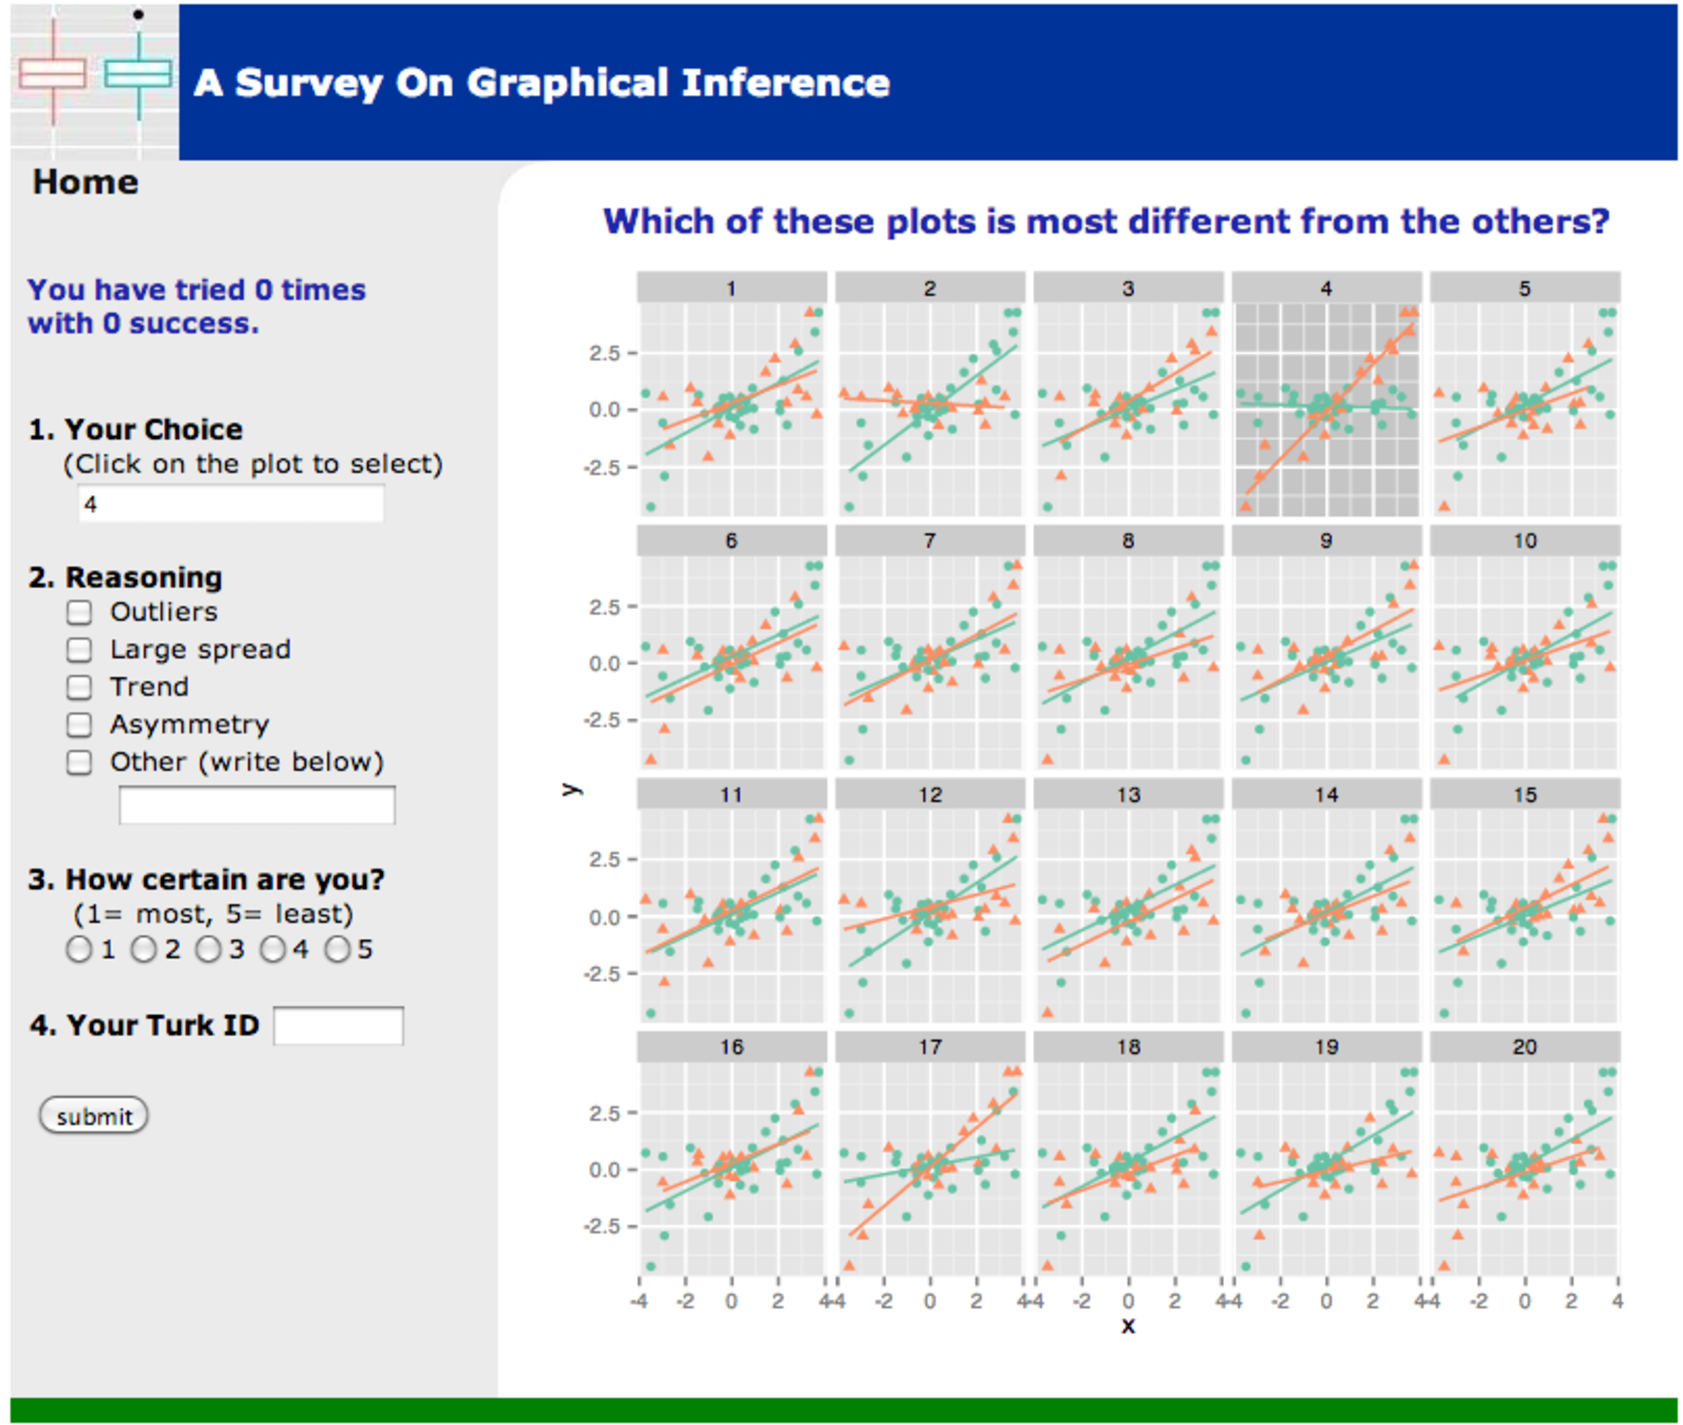
\includegraphics{turk_web.pdf}}
       \caption{A sample data collection form. Lineups are presented at random for evaluations by the turk workers. Scalable Vector Graphics (SVG) is used so that observer can click on the lineup to pick certain plot. Once a plot is selected it gets shaded and the number appears in the choice text box.}
       \label{fig:turk_web}
\end{figure}

One of the nice features of the form in Figure \ref{fig:turk_web} is the use of Scalable Vector Graphics (SVG) for lineup which enables an observer to give feedback with the ease of just a mouse click. If the observer changes mind he or she can click the plot again and deselect it. If needed multiple selection of plots can be allowed, order of selection and deselection can be recorded with time taken for each action. Thats what we meant by saying it is complex in design. 

It is possible to let workers see the statistics of their total feedbacks with number of correct evaluations. This feature can be opted out easily if not necessary. The workers have to provide their turk ID and for next evaluation they don't have to type it again. This allows the worker give feedback using only mouse click. Thats what we meant by saying it is simple for turk worker.

Once the data is submitted a feedback can be provided whether their choice was correct or wrong. This feature can also be opted out easily if not needed. The design of the feedback form is shown in Figure \ref{fig:turk_web_feedback}. This form is also used to collect demographic and educational information about the worker. After the required number of evaluations are obtained, a pass code is given as a proof of the completion of the task which is used for payment purpose later.

\begin{figure}[hbtp]
   \centering
       \scalebox{.4}{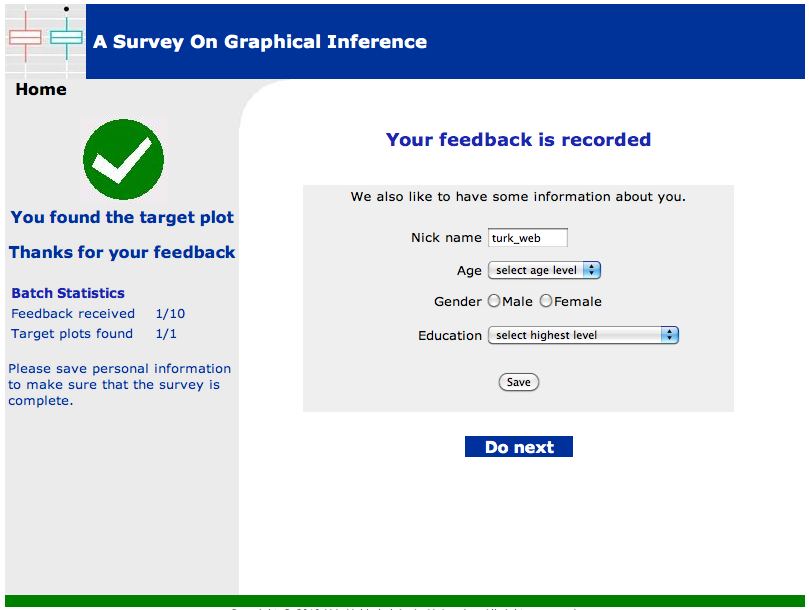
\includegraphics{turk_web_feedback.png}}
       \caption{The turk workers are given feedbacks whether their evaluation for each lineup was correct or not. This works as an incentive for the worker to work more enthusiastically. To ensure the payment, the turk workers have to provide some information using this form.}
       \label{fig:turk_web_feedback}
\end{figure}

Each worker is shown some specific number of lineups for evaluation. These lineups are randomly selected from a pool of lineups designed for evaluations. The algorithm for how the lineups should be selected to show and what would be the order of display is implemented in the form shown in Figure \ref{fig:turk_web}. Also there is a check for invalid or missing information which is implemented using javascript. If users try to go forward without giving any feedback they are not allowed to do that showing a warning message.

%After the evaluation is recorded on a lineup through form shown in Figure \ref{fig:turk_web} another form shown in Figure \ref{fig:turk_web_feedback} is used to give feedback to the turk users whether they correctly identifies the true plot and how many evaluations are recorded from the users. 


\subsection{Database design} The design of the database to store the collected data is shown in Figure \ref{fig:turk_database_design}. It is designed such a way that data from many different experiments can be stored in the same database. In total five separate tables are used. Table turk\_worker contains static information about each turk worker. The location information of each turk worker is stored in ip\_detals table. The information in this table is collected later based on the ip address of each turk worker. Table picture\_delais contains the static information about each lineup. Table feedback is a dynamic table that grows with the number of feedbacks from each turk worker. The multiple activities of the worker are recorded in turk\_activity table. This table also contains the codes provided to the workers once they finish the experiment. 

\begin{figure}[hbtp]
   \centering
       \scalebox{.4}{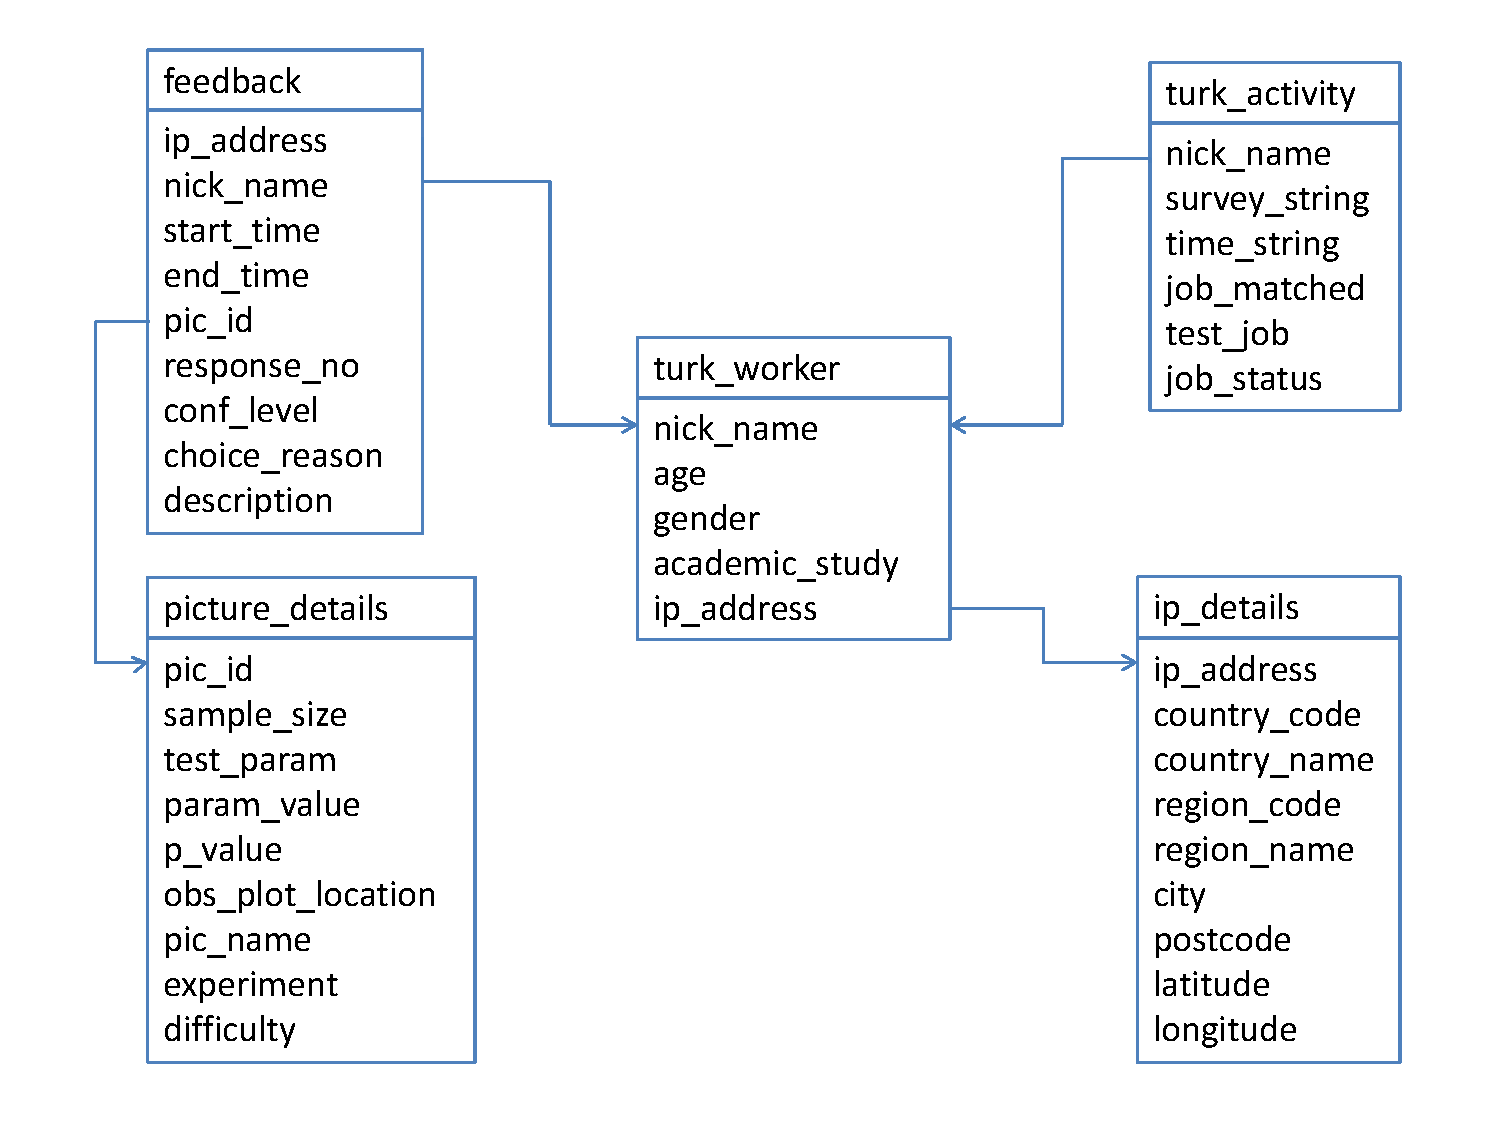
\includegraphics{turk_database_design.pdf}}
       \caption{Relational database design for MTurk experiment data collection. The same database can be used for multiple turk experiments by keeping experiment information in picture\_details table which contains information about the lineups.}
       \label{fig:turk_database_design}
\end{figure}

The primary key in feedback table is produced by nick\_name and pic\_id since no workers are allowed to provide multiple feedbacks on the same lineup. In all other tables the first field names shown in Figure~\ref{fig:turk_database_design} are the primary keys. For the implementation of the web application we used MySQL database located on a local server.

\subsection{Data collection} 

The homepage of the web displays detailed explanation on how one can perform the task of evaluating the lineups. Several examples with possible answers are provided. It is possible to customize how the workers will proceed from the home page. There are two options; one is to allow them to continue the task where no trial is needed. The second option is to force them to try some lineup before joining the actual experiment. The trial feedbacks are not recorded. As per the requirement of Institutional Review Board (IRB) the workers need to provide the informed consent. For this they have to read and agree with specific IRB approved informed consent. The flow chart for this data collection sequence is shown in Figure \ref{fig:turk_data_flow}.

\begin{figure}[hbtp]
   \centering
       \scalebox{.4}{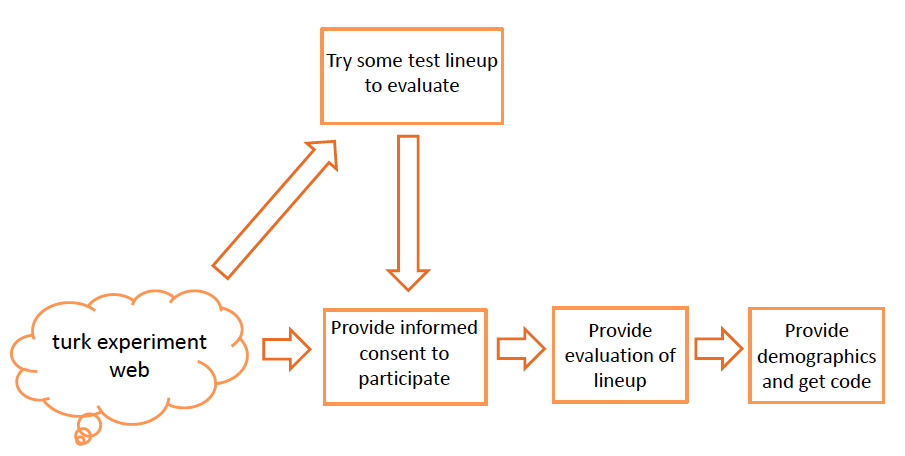
\includegraphics{turk_data_flow.png}}
       \caption{Data collection work flow shows that workers can try some test lineups before going to the live experiment after providing informed consent. This design gives the flexibility to make the trial mandatory, if needed, so that without having enough correct trial evaluations the actual participation can be prevented.}
       \label{fig:turk_data_flow}
\end{figure}


%To collect the survey data we developed a web site that shows a plot to an individual and get feedback from that individual. Each individual is asked to provide feedback for at least 10 different plots. The 10 plots that are shown to an individual are randomly chosen with probability proportional to the number of responses required (the sample size) for that plot.

%The MTurk workers were redirected to the web site and the data were collected, stored automatically into a local database server. Demographic informations such as age group, gender and education levels were also collected. The time taken for each evaluation is computed based on the time the plot was shown and the time the feedback was received. The location of the observer is determined by the ip address of the observer.

%Figure \ref{fig:turk_work_flow} turk workers have to visit the experimental web site and give their consent to participate the survey as per IRB requirement. In the experimental web, there is a option for observers to try some sample lineups to get familiar with the experiment. Once the observers start evaluating the lineups they are sequentially shown a specific number of lineups and at the end they are given a code as a proof for their tusk completion. The payment of the turk worker is processed if they post the code they got from experimental web site. The observers are also asked to provide some demographic information about them to make sure that the code is generated.

The default information that the system is designed to collect from each individual is shown in Table \ref{tbl:data_info}. Data received from each individual will be automatically saved in a secured mysql server. 

\begin{table}[hbtp]
\caption{Default information the web application collects from each individual}
\centering 
\begin{tabular}{lp{8cm}} 
\hline
Information &  Description \\ %[0.5ex] % inserts table %heading 
\hline
Identification & Nick name or any ID to determine the responses of an Individual \\
Response number & The number of the plot on the lineup plot which the individual thinks the most different than other 19 plots.\\ 
Reason of of choice & Reason why the individual chooses the plot \\
Confidence level & Confidence level of individual choice \\ 
Age group& The age group where the individual belongs \\
Education & The highest level of education completed \\
Gender & Male or female \\
Geographic Location & This information is collected through the ip address of the individual computer \\ 
Time taken & Time taken for each response\\
\hline
\end{tabular}
\label{tbl:data_info}
\end{table}	


%\subsection{Data collection sequence} 


\subsection{Data Security and Validity} 

Since the experiment is based on online participations and related to monetary affairs, it is important to maintain certain security for the data collection. The attempt to provide random data or irrelevant information as well as harmful actions need to be prevented.  Some cautious attempts are taken to add security to the data. Server side scripting language PHP is used to connect to database and access or save data. For transferring data from one form to another PHP session variables are used. Cookies are avoided carefully so that no important informations are saved in the cookies. 

To prevent missing information and invalid input client side controlled is applied using JavaScripts. Most of the cases options or combo boxes are used instead of free text boxes to avoid invalid input. This also made the task easy to perform and convenient for the workers. For controlling some flow of the work such as showing various messages, JavaScripts are used as well. Careful consideration are made so that no important informations are stored in the java variable or function that could easily be revealed.


\section{Managing Turk Task}\label{sec:turk_task} \cite{turk} Mechanical Turk website provides various features that are helpful to maintain and organize the task and manage the workers. Creating, posting, accepting or rejecting tasks and processing payment are done from the MTurk system. It is also possible to screen out workers as needed. For example, none will be interested to recruit people who have a very bad reputation. This information can be obtained from each worker's previous work history of total number of accepted task out of total number of submitted task. The web application we developed is for presenting lineups in a flexible way the researcher may want  as per the experimental design and collecting data. To get people to the web application we need to design a turk task in MTurk system.

%Turk workers are usually small payee workers. There are several issues related to the payment of their effort. These are briefly discussed in the following section. 

% and we intend to work more on this as we progress through this dissertation work. 

\subsection{Creating Task for Lineup Evaluation} To create a MTurk task some parameters have to be specified. The task descriptions need to be as simple as possible. This description makes the first impression about the task along with the amount of money to be paid for each task. Once the worker agrees to do the task they may come to the web site designed for lineup evaluation. Thus it is important to provide them with enough information so that they don't have to spend much time after coming to the web application. Some other parameters that need to be specified are discussed below.

\begin{itemize}

\item The number of worker to recruit has to be provided so that the turk task remain open until specific number of people do the task. This is related to the sample size of the data we intend to collect on each lineup. 

\item Time allowed to finish each task has to be specified. Once a specific time period is set up the task will be expired after that time and the worker can't submit it anymore. The worker has to finish the task by that time period once he or she agrees to do the task. 

\item Qualifications needed to view and perform the task may be specified so that only desired participants can do the task. It depends on the population of interest as per the experimental design. For example one may only allow workers who have a history of doing at least 100 tasks and out of which a specific percent of tasks have been approved by other recruiters. 

\item Duration of the task is the period of time the task is available for workers to do. If the time period is over the task will not be available no matter whether all the required number of workers have participated or not. This duration is important as each payment has to be finalized by this time period. Otherwise, all the workers will be paid automatically after this time period no matter whether the the task is accepted or rejected. Some times it is helpful to set up a longer duration and see how long it takes before all the tasks get completed.

\item Finally, the workers are redirected to the web site designed for lineup evaluation. MTurk workers should be informed clearly that they will be redirected to a new website from where they will provide feedback. The whole task including the instructions and procedures in the web application should be presented as per the task plan described in Section \ref{sec:task_plan}.

\end{itemize}

\subsection{Accepting or Rejecting the Task} There is no hard and fast rule to follow while accepting or rejecting the tasks submitted by the MTurk workers. Since MTurk task are very simple and payment amount is very small the general convention is to pay every worker who submitted the task properly as instructed. The task should not be rejected based on the quality of work unless it clearly demonstrates that the task was not performed properly and irrelevant or garbage data were provided. It is very unusual to get garbage data from MTurk workers since they are well aware that this conduct may harm their reputation as a worker. So, proper caution needs to be taken while rejecting a task. Some times it may happen that the workers provided invalid data unintentionally. In that case we recommend to accept the task and pay for trying the task.

It is very difficult to detect whether a worker is giving data by properly inspecting the lineup or just at random. This can be monitored by putting a test lineup which is very easy to evaluate. The worker can be informed that there will be a test lineup which need to be correctly evaluated to make sure the task is accepted. This may prevent worker giving random data and it is easier to accept or reject tasks based on this criteria.  

There may be mistakes made by the worker such as giving a wrong ID or a invalid input even though the whole task is properly done as instructed. In this case the task should be accepted and payment should be made. This encourages the workers and they appreciate the recruiters sincerity and provide good feedbacks. This does not happen frequently if qualified workers are recruited such as who had at least a certain number of percentage of tasks approved previously. 

Other criteria to accept or reject the tasks may be more complex based on the experimental needs. For example one may accept the task if certain percentage of the easy lineups are correctly evaluated. This criteria can be used if multiple number of easy lineups are shown for evaluation. For example if there are 3 easy lineups and none of them were correctly evaluated it is most likely that the feedbacks were provided randomly. Some times it may happen that out of 10 lineups 3 difficult lineups were correctly evaluated but all the three easy lineups were wrongly evaluated. In that case the payment should be made since it is very unlikely that out of 10 lineups a total of 3 lineups would be correctly evaluated by just random response.
%These issues would be addressed in our future work based on the several turk experiments that we intend to carry out.

The payment of the workers is directly associated with the rejection of the work. If the task is not accepted the payment to the worker is denied and reasons for rejecting the tasks should be clear so that the worker doesn't get confused.

%\subsection{Payment for the Worker}Amazon Mechanical Turk suggests that each worker gets \$6/hour as wage. Thus we need to estimate how much time a task may take to complete and based on that we have to specify the payment for each task. Our experience indicates that a better payment brings more serious workers who usually provide cleaner data which is more reliable. 

%We may study this issue while we do multiple turk experiments.

\subsection{Managing Worker} Accepting the task and processing the payment in a timely manner may make a good impression about the task and the recruiter. This is helpful for the recruiter's reputation so that in future the recruiter can get the job done faster. Since the MTurk worker will always  prefer the tasks posted by a good recruiter. Besides this we provide some good worker management strategy as below.

\begin{itemize}

\item Not all the workers put the same effort while doing the task. Some workers spend much time and perform the task sincerely and follow the instructions very carefully. That effort is observable in their responses and time taken for each evaluations as well as from the textual feedbacks such as writing choice reasons in details. We recommend paying bonus to those workers in addition to the regular payment. 

\item If a work is not worth paying bonus payment we still recommend to appreciate each work. Even when the task gets rejected a proper explanation of rejection along with an appreciation for at least trying to participate the experiment is very useful for a recruiter's good image. 

\item Some workers may email to learn more about the experiment. Some times they may face technical troubles which needs to be taken care of promptly. A timely communication with worker is necessary and emails should be responded as  promptly as possible. It is important as they can report any trouble to IRB which may create unpleasant issues with the human subject experiment.

\item It is recommended to reject the task if it is not submitted as requirement. Some times this may produce dispute and the workers may become angry and demand payment. We recommend to be strict to the decision and for any further administrative control there is an option to block the worker if necessary. After all this is a work place and it is expected that the worker maintain the work place environment.

 \end{itemize}

\section{Turk Experiment Data} \label{sec:turk_data}

We have performed 10 different experiments using the web application described in Section~\ref{sec:web_application}. Table~\ref{tbl:mturk} presents the tasks and payment details of all the 10 experiments. Experiment 1 was the first experiment and the largest number of tasks were rejected in that experiment. But this experiment provides valuable information about how to modify the web site to avoid invalid input and missing information. Thus in the later experiments we did not see a lot of tasks to get rejected.

\begin{table}[hbtp]
\caption{Amazon mechanical turk experiments and their properties. Duration in hours per 100 tasks show the popularity of some tasks compared to others.}
\centering
\scalebox{0.85}{
\begin{tabular}{rlrrrrrrr}
  \hline
& Experiment& \multicolumn{2}{c}{ Total Task}& Average & \multicolumn{2}{c}{Duration (hour)} & Payment & Pay rate\\
\cline{3-4} \cline{6-7}
Serial & description & submitted & rejected & time(min) & Actual & 100 task& \$/task & \$/hour\\ 
  \hline
1 & Boxplot & 406 & 106 & 10.68 & 146.48 & 36.08 & 0.50 & 2.81 \\ 
  2 & Scatterplot & 359 &   9 & 10.80 & 42.68 & 11.89 & 1.00 & 5.58 \\ 
  3 & Contaminated plot & 219 &  19 & 13.53 & 126.17 & 57.61 & 1.00 & 2.22 \\ 
  4 & Polar vs Cartesian & 110 &  10 & 20.65 & 11.65 & 10.59 & 1.00 & 2.91 \\ 
  5 & Hist vs density & 234 &  37 & 17.85 & 41.57 & 17.76 & 1.00 & 3.36 \\ 
  6 & Violin vs boxplot & 417 &  17 & 17.95 & 105.87 & 25.39 & 1.00 & 3.34 \\ 
  7 & Group separation & 106 &   6 & 16.13 & 5.15 & 4.86 & 1.00 & 3.72 \\ 
  8 & Sine Illusion & 101 &   1 & 16.52 & 78.38 & 77.60 & 1.00 & 3.63 \\ 
  9 & Gene expression & 103 &   3 & 12.47 & 11.27 & 10.94 & 0.50 & 2.41 \\ 
  10 & Test normality & 406 &   6 & 22.70 & 74.35 & 18.31 & 1.00 & 2.64 \\ 
   \hline
\end{tabular}
}
\label{tbl:mturk}
\end{table}

The hourly payment rates shown in Table~\ref{tbl:mturk} are based on the time periods beginning from the times the tasks were accepted by the worker to the time they were submitted to the MTurk system. It is different from the time taken to actually evaluate the lineups. Since in between the workers need to go to the web application, get the codes after they finish the tasks and finally put the code to MTurk system. The pay rate is almost similar for all the experiment except for experiment 2. The payment was decided based on the MTurk standard of \$6 per hour and we can see that for experiment 2. Based on the experiment 1 and 2, they payment for each task was fixed to \$1, but in practice, it appears to be much less than that. It is because, workers spent long time in between lineups.

%In this section we intend to analyze the performance of the experiments we did using Amazon Mechanical turk. We have feed back data for the similar plots from both turk workers as well as from the people who regularly participates in the graphics group meeting of our department. We consider later participants as more knowledgeable and trained in seeing pattern in statistical plots. We can use these data to evaluate the performance of the general participants from around the world.

The duration of an experiment to finish depends on the time it was posted and the number of interested workers available on that time. It also depends on how attractive the experiment is in terms of appearance and payment. Even though the payment was similar for all the experiments, we observed some experiments were finished much faster than others. Experiment 8 took long time to finish which is about 77 hours for 100 tasks while experiment 7 took only 4.86 hours to finish 100 task.

Figure~\ref{fig:task_duration} shows the comparative durations of time for 100 tasks in each of the experiment. Even though experiment 8 (sine illusion) took longer to finish it got the least number of rejected tasks.



\begin{figure}[htbp] 
   \centering
   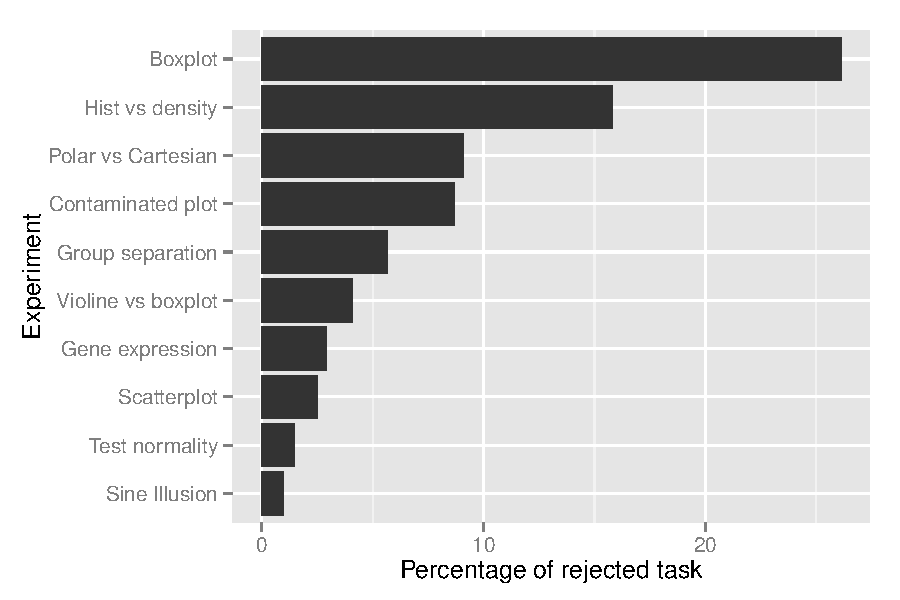
\includegraphics[width=3in]{rejected_task.pdf}
      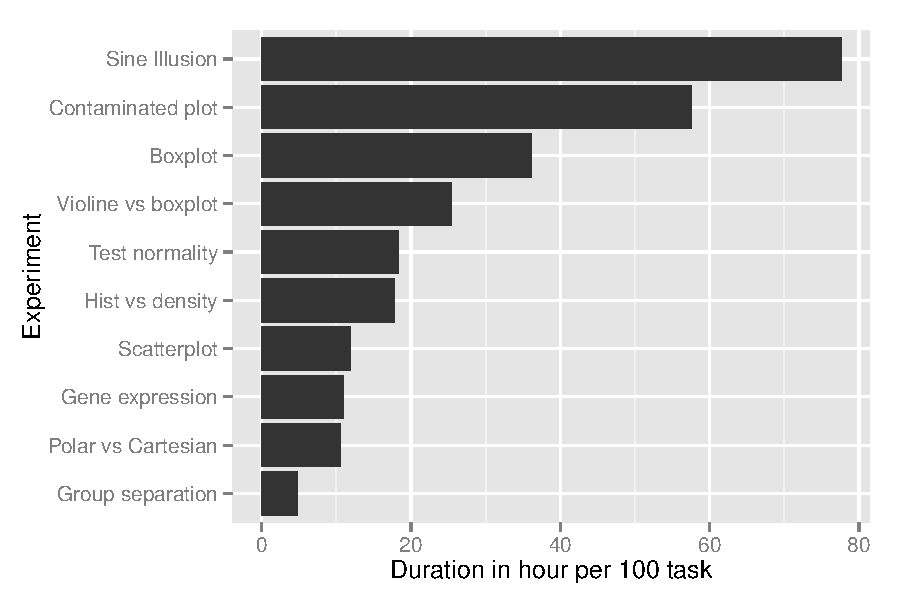
\includegraphics[width=3in]{task_duration.pdf} 
   \caption{Percentage of rejected tasks and duration of each experiment in hour per 100 tasks for each of the 10 experiments. Most of the tasks got rejected for box plot experiment.  Even though the sine illusion experiment took longest to finish the rejection rate is lowest for this experiment.}
   \label{fig:task_duration}
\end{figure}


\subsection{Data Cleaning} Data cleaning is different than accepting and rejecting the task. There may be some tasks for which payment is provided but yet the tasks may need to be excluded from the study. It is because there may be some participants who did not put in a best effort to identify the data plot in the lineup, but just randomly picked a plot to maximize their 'winnings'. We present following six suggestions about cleaning data from turk experiments where each worker evaluates multiple lineups.  

\begin{enumerate}
\item {\bf include all participants} and their evaluations
\item exclude all participants' evaluations, who did {\bf not} share their {\bf demographic information} (age, gender education level -- all three pieces of information are either missing or all present).
\item exclude participants' records, if {\bf none of the evaluations}  correctly identified the data plot -- every participant was shown a range of `easy' lineups.
\item include participants' records, if   {\bf at least 20 percent} of the evaluations are {\bf correct}  -- based on ten evaluations per participants, two correct evaluations are significant evidence against a person just guessing
\item include participants' records, if at least {\bf 50\% of all very easy lineups are correct} 
\item use easy lineups as {\bf reference charts}: sample one easy lineup from a person's records. If that lineup is evaluated {\bf correctly}, include all (other) lineups of that person, otherwise exclude all lineup evaluations by this participant.
\end{enumerate}

These screening criteria may be applied based on the specific design of the study and experimental evidence. For example \cite{majumder:2013} used criteria 6 to clean the data.

%Amazon Mechanical Turk data suffers from the problem that some participants are trying to 'game' the system, because they are being paid for their efforts, not much by the standards of the US minimum wage, but enough to encourage honest efforts.  in our situation, these are participants who did not put in a best effort to identify the data plot, but just randomly picked a plot to maximize their 'winnings'.  In order to avoid using those results, we are comparing six different screening methods for excluded participants from the data analysis.  There are six suggested approach to clean the data.  They are




%\subsection{Diversity in the Data} Demographics, geographical locations, academic diversity

%\begin{figure}[hbtp]
%   \centering
%       \scalebox{.5}{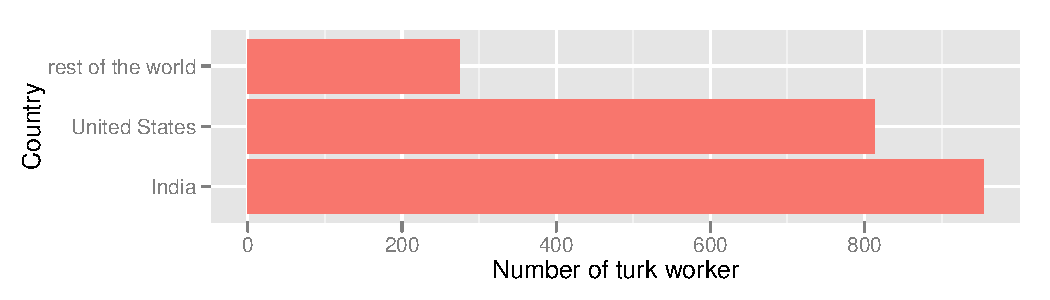
\includegraphics{turker_country.pdf}}
%       \scalebox{.5}{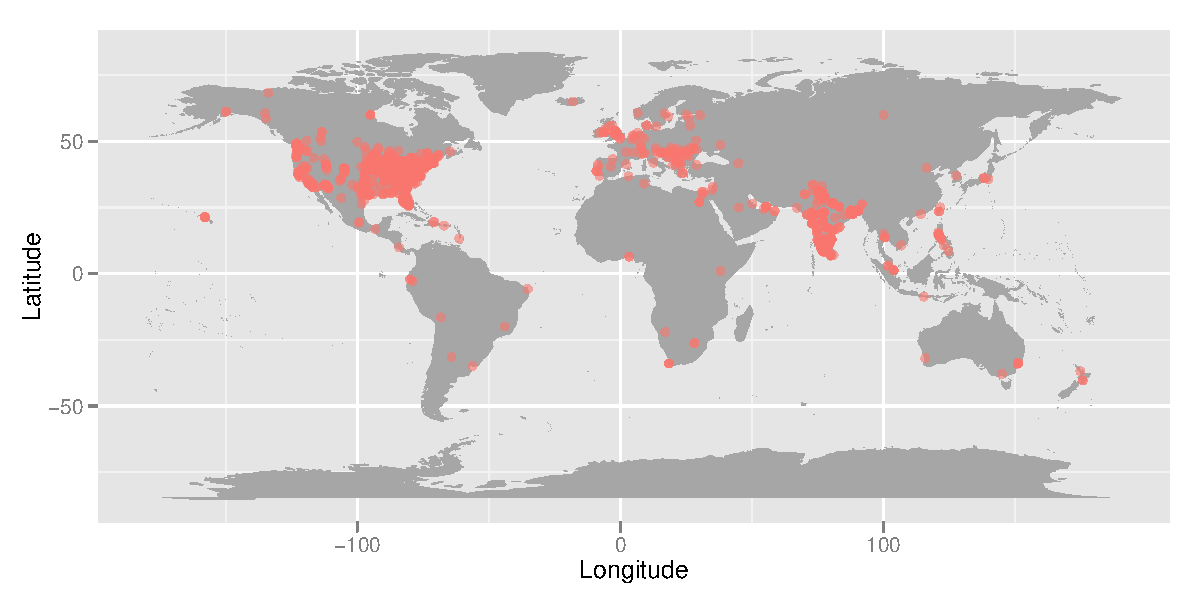
\includegraphics{turker_location.pdf}}       
%       \caption{The location of turk workers on the world map shows the geographical diversity of turk workers even though most of the workers come from India and United States.}
%       \label{fig:rsq}
%\end{figure}

\subsection{Selection Bias} 

%Since data are collected through web interface it is possible to have the selection bias in the turk experiment we did. In this section we intend to analyze to what extent this selection bias has occurred and how we can adjust for this.

There is always a concern of selection biases with any online study. First of all in online study only those who use internet can participate. For a turk experiment the pool of participants even shrinks further to those who work in MTurk system. 

Other biases may be due to the time the task is posted online, setting up specific qualification or even payment amount. A task which is posted at noon in central time in USA is less likely to be seen from Indian region since that is the midnight in that area. This may produce an artificial filter to the data which may come only from certain geographical location. If a specific qualification of the task is required not all the workers are able to view and perform that task. Also, if payment amount is very small many worker may not even review the task.  

While selection bias may influence the results of some experimental study it is not much of an issue for experiment with lineups. In terms of demographic factors and geographic location MTurk provides much diversity in the participants as studied by \cite{majumder:socio}. Moreover it is observed that the human factors do not have any practical impact on the probability of correctly identifying the data plot in the lineup. 



% may recruit from a specific geographical location

%Setting up qualification may allow certain workers to do the task

%Payment amount may affect the duration of the experiment which may avoid diversity in the geographical locations.


\section{Conclusion} This paper presents a complete solution to the problem of designing a simulation experiment for lineup and recruiting people to get the lineups evaluated. The online application design provides features to control how the multiple lineups can be presented to an observer. Scalable Vector Graphics (SVG) are used for lineup so that observer can click on the lineup to pick certain plot. This also made the multiple plot selection from a lineup easier and convenient. The web site is used for multiple online experiments.

One of the main features of the web application is that it produces simple task for the worker but still retains many flexibilities to the researcher who need lineups to be evaluated as per complex experimental requirement. The design of this application allows recruiting people from any source not necessarily just from MTurk. The web application is now hosted on Iowa State University public domain \citep{majumder:turk} and any number of experiments can be done through this web site without changing the core of this application.

The next direction of this work is to make a complete package so that anyone can reproduce this web application, customize according to their need and run the MTurk experiments as part of their research that involves lineups. This will also help lineup protocol to be used frequently since it will provide an ease of its use in making inferential decisions.

We also intend to set up a web application for public use where researcher can put their lineup for online evaluation. The observer can be recruited from MTurk or any other sources including local lab participants. 

\paragraph{Answer to the question in Figure~\ref{fig:lineup_turk} is 2.}


%
%\section{Appendix: What do Turk Workers Pick, $R^2$ or $p$-value?} What do people pick in a lineup plot, p-value or $R^2$? To address this issue we obtain the approximate theoretical relationship between $R^2$ and the power of the classical hypothesis test. Suppose we want to test the significance of the slope ( i.e.,  $H_0: \beta=0$ against $\beta \ne 0$) of a continuous covariate $X$ in  a simple linear regression model setting. Also consider $X \sim N(0,1)$. For a sample of size $n$ this gives us 
%\begin{eqnarray*}
%Y_i-\bar{Y}& = & \beta_0+\beta_1X_i+\epsilon_i - \beta_0 - \beta_1 \bar{X}- \bar{\epsilon} \\
%          & = & \beta_1(X_i-\bar{X})+(\epsilon_i-\bar{\epsilon})
%\end{eqnarray*}
%Now 
%\begin{eqnarray*}
%X_i-\bar{X}& = & X_i - \frac1n (X_1 + X_2 + ... + X_i + .....+ X_n) \\
%          & = & X_i - \frac1n X_i - \frac1n \sum_{j \neq i}{X_j}\\
%          & = & (1-\frac1n)X_i - \frac1n \sum_{j \neq i}{X_j}
%\end{eqnarray*}
%
%Thus we have 
%\begin{eqnarray*}
%E(X_i-\bar{X})^2 & = & (1-\frac1n)EX_i^2 - \left( \frac1n \right )^2 (n-1) EX_j^2 \\
%                 & = & (1-\frac1n)^2+ \frac{n-1}{n^2}\\
%                 & = & \frac{n-1}{n}
%\end{eqnarray*}
%
%Similarly we have 
%
%\begin{eqnarray*}
%E(\epsilon_i-\bar{\epsilon})^2 & = & (1-\frac1n)E\epsilon_i^2 - \left( \frac1n \right )^2 (n-1) E\epsilon_j^2 \\
%                 & = & \left((1-\frac1n)^2+ \frac{n-1}{n^2} \right) \sigma^2 \\
%                 & = & \frac{n-1}{n}\sigma^2
%\end{eqnarray*}
%Finally we have expected total sum of square (SST) as
%\begin{eqnarray*}
%E\sum_i{(Y_i-\bar{Y})^2} & = & \sum_i E(Y_i-\bar{Y})^2=\sum_i \left [ \beta_1^2 E(X_i-\bar{X})^2 + E(\epsilon_i-\bar{\epsilon})^2 \right] \\
%                 & = & \sum_i\left[ \beta_1^2 \frac{n-1}{n}+  \sigma^2 \frac{n-1}{n}\right]\\
%                 & = & (n-1)(\sigma^2+\beta_1^2)
%\end{eqnarray*}
%
%We know $E(MSE|X) = \sigma^2$ or $E(SSE/n-2)|X = \sigma^2$ which gives the expected residual or error sum of square as $$E \sum_i (Y_i-\hat Y_i)^2=(n-2)\sigma^2$$
%Thus we have the expected regression sum of squares $SSR =  (n-1)(\sigma^2+\beta_1^2) - (n-2)\sigma^2 = (n-1) \beta_1^2+\sigma^2$ This gives $$R^2=\frac{(n-1) \beta_1^2+\sigma^2}{ (n-1)(\sigma^2+\beta_1^2)}$$
%
%
%\begin{figure}[hbtp]
%   \centering
%       \scalebox{.3}{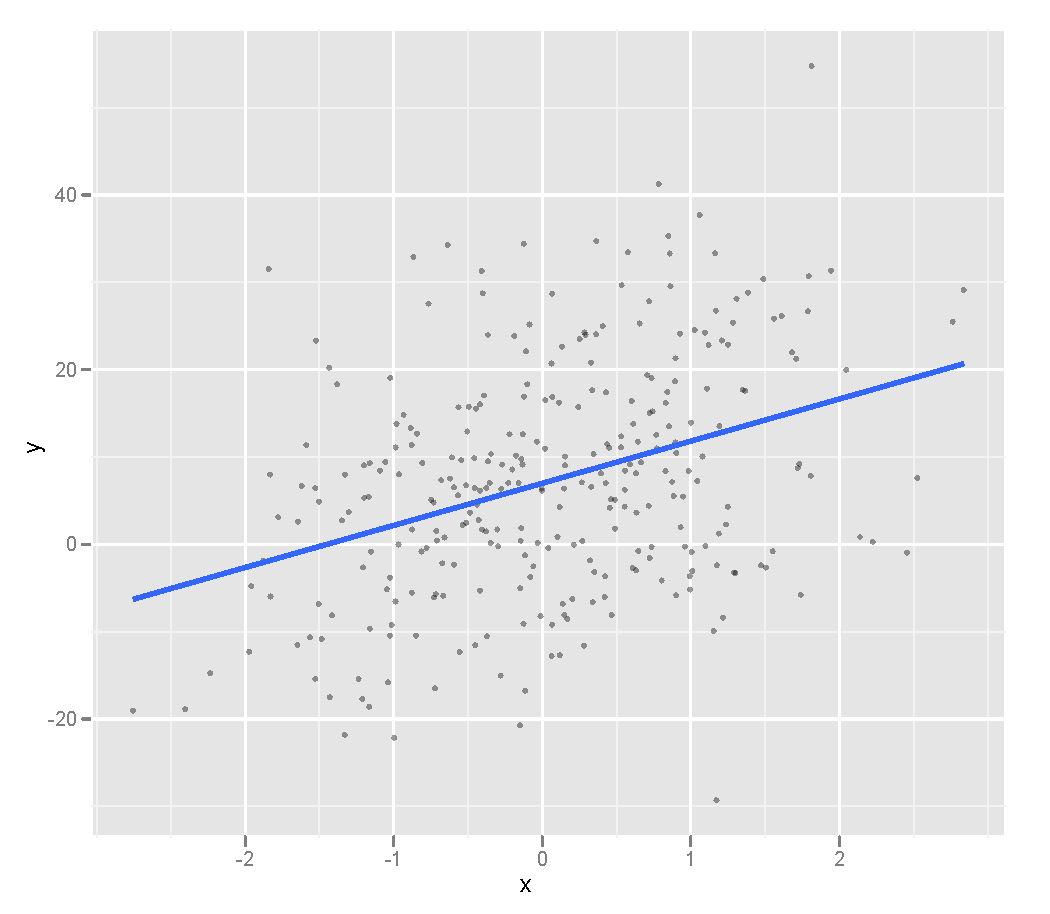
\includegraphics{scatter_plot_beta_4.pdf}}
%       \caption{Scatter plot of data generated for $\beta_0$=6, $\beta_1$=4, sample size $n =300$ and $\sigma = 12$. $R^2$ for this data was obtained as 0.1309 showing that the model could not successfully explain the variation in $Y$. But notice in figure \ref{fig:power_rsq} that power for $\beta$=4 is almost 1. So, Can we conclude that $R^2$ does not have any effect in deciding whether $H_0: \beta_1=0$ should be rejected or not?}
%       \label{fig:plot_beta_4}
%\end{figure}
%
%
%\begin{figure}[hbtp]
%   \centering
%       \scalebox{.35}{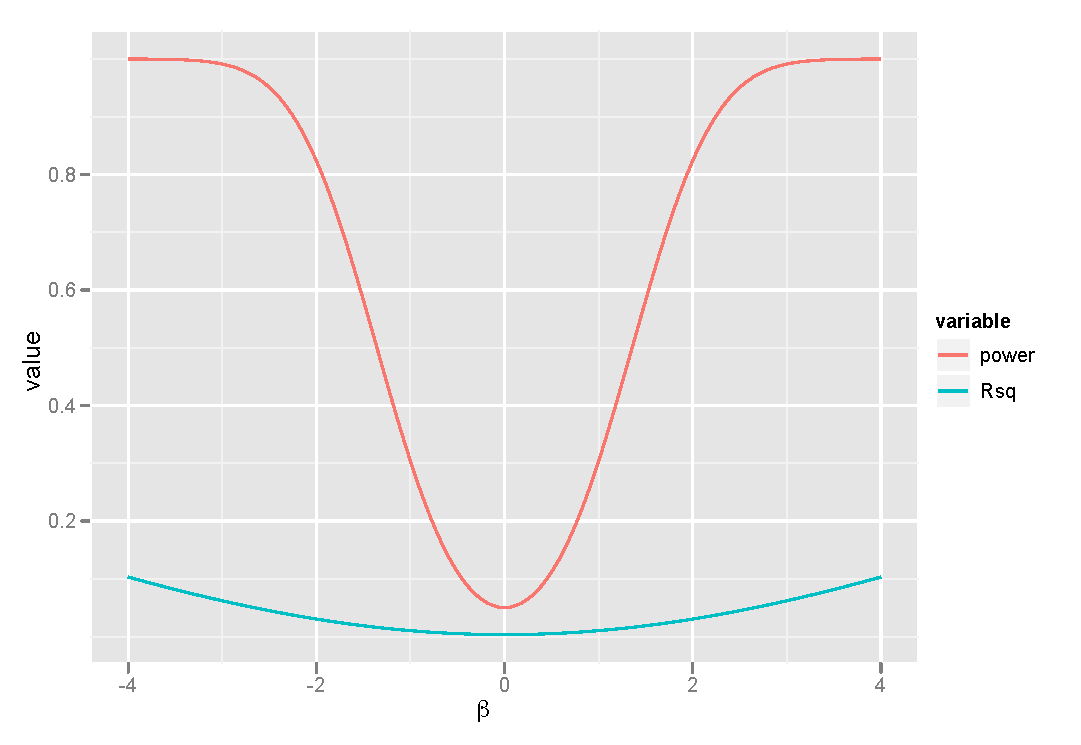
\includegraphics{power_300_12.pdf}}
%       \caption{Power curve and $R^2$ values for sample size $n =300$ and $\sigma = 12$. Notice that for a small value of $R^2$ (0.1) the power is almost 1.}
%       \label{fig:power_rsq}
%\end{figure}
%
%
%\begin{figure}[hbtp]
%   \centering
%       \scalebox{.35}{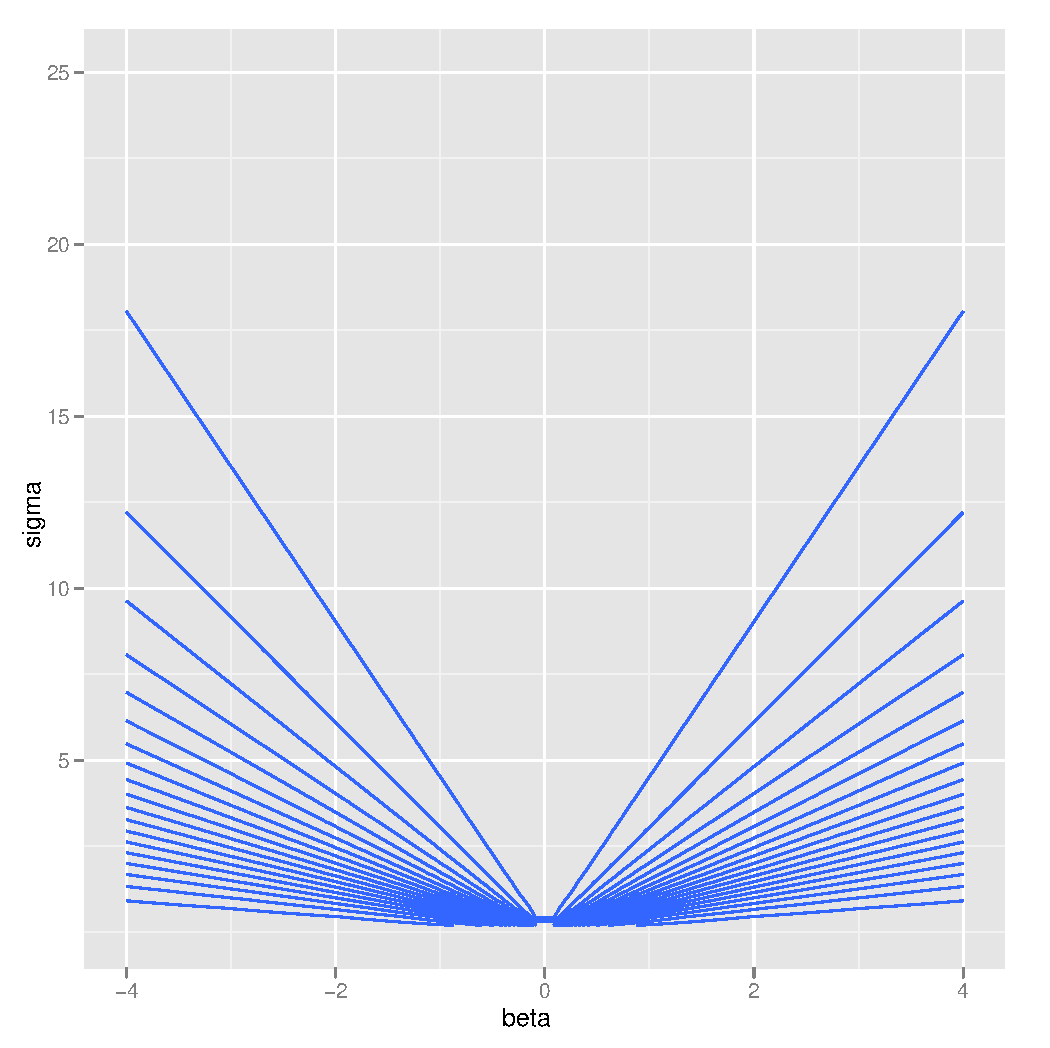
\includegraphics{rsquare_contour.pdf}}
%       \scalebox{.35}{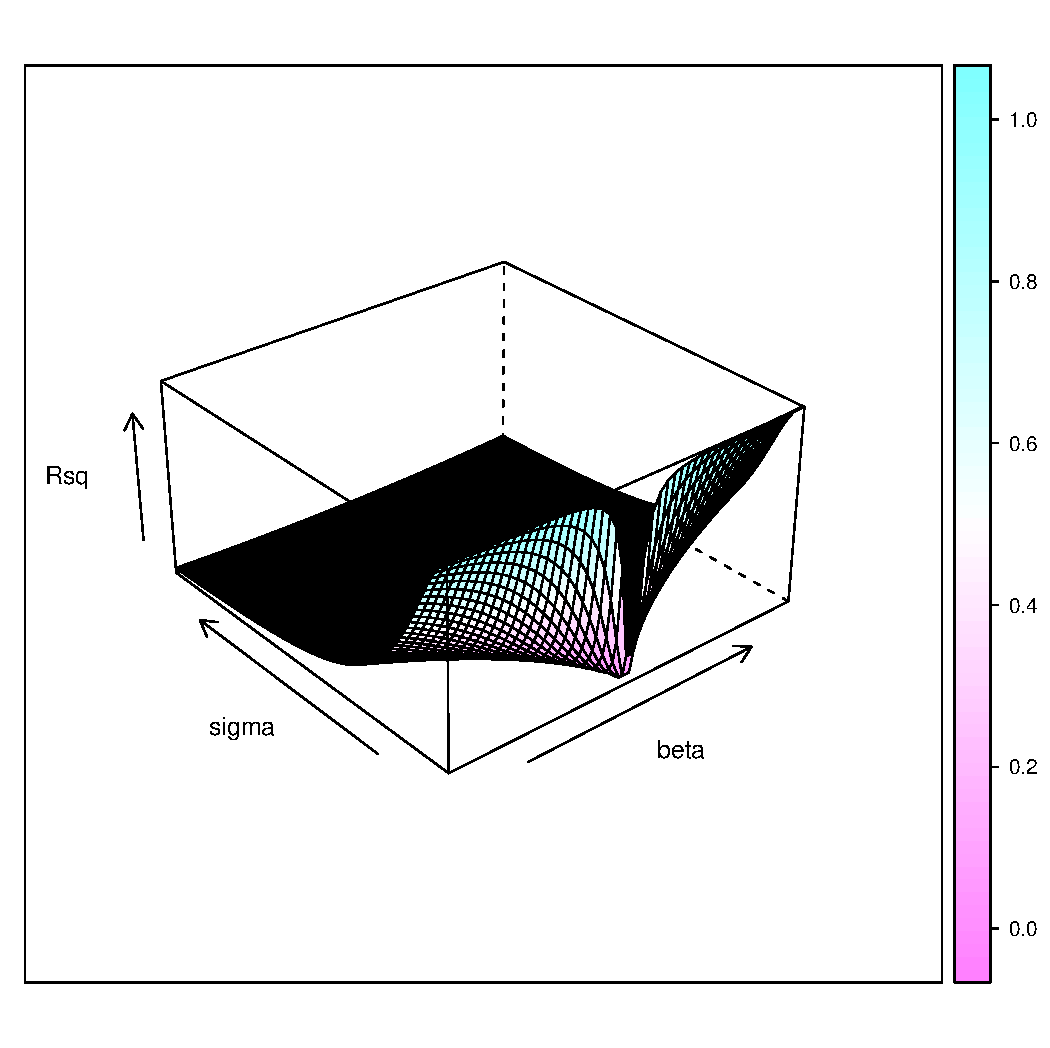
\includegraphics{rsquare_beta_sigma.pdf}}
%       \caption{Contour and surface plots of $R^2$ for sample size $n =300$. The values for $R^2$ goes down sharply with $\sigma$ and $\beta$.}
%       \label{fig:contour_rsq}
%\end{figure}
%
%\begin{figure}[hbtp]
%   \centering
%       \scalebox{.35}{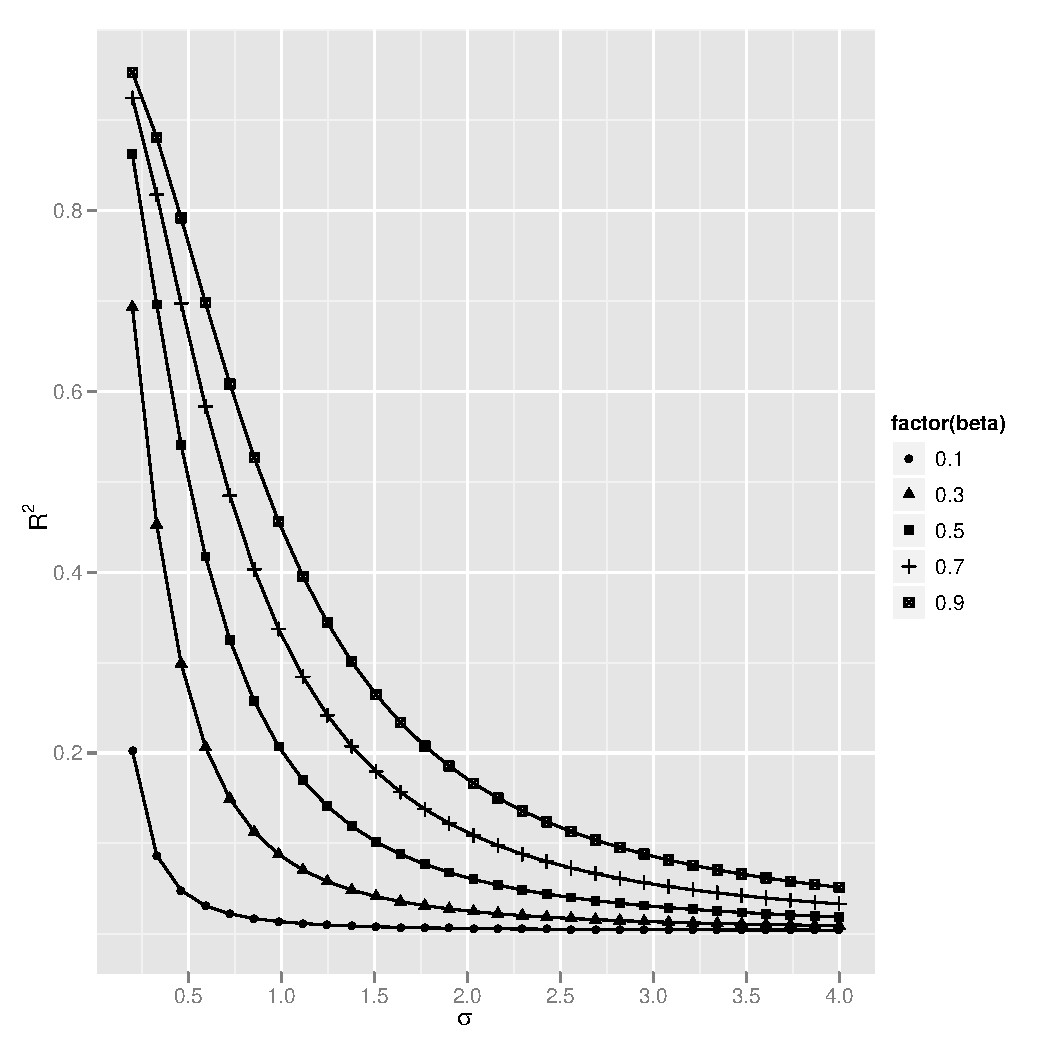
\includegraphics{rsquare_beta_sigma_lines.pdf}}
%       \scalebox{.35}{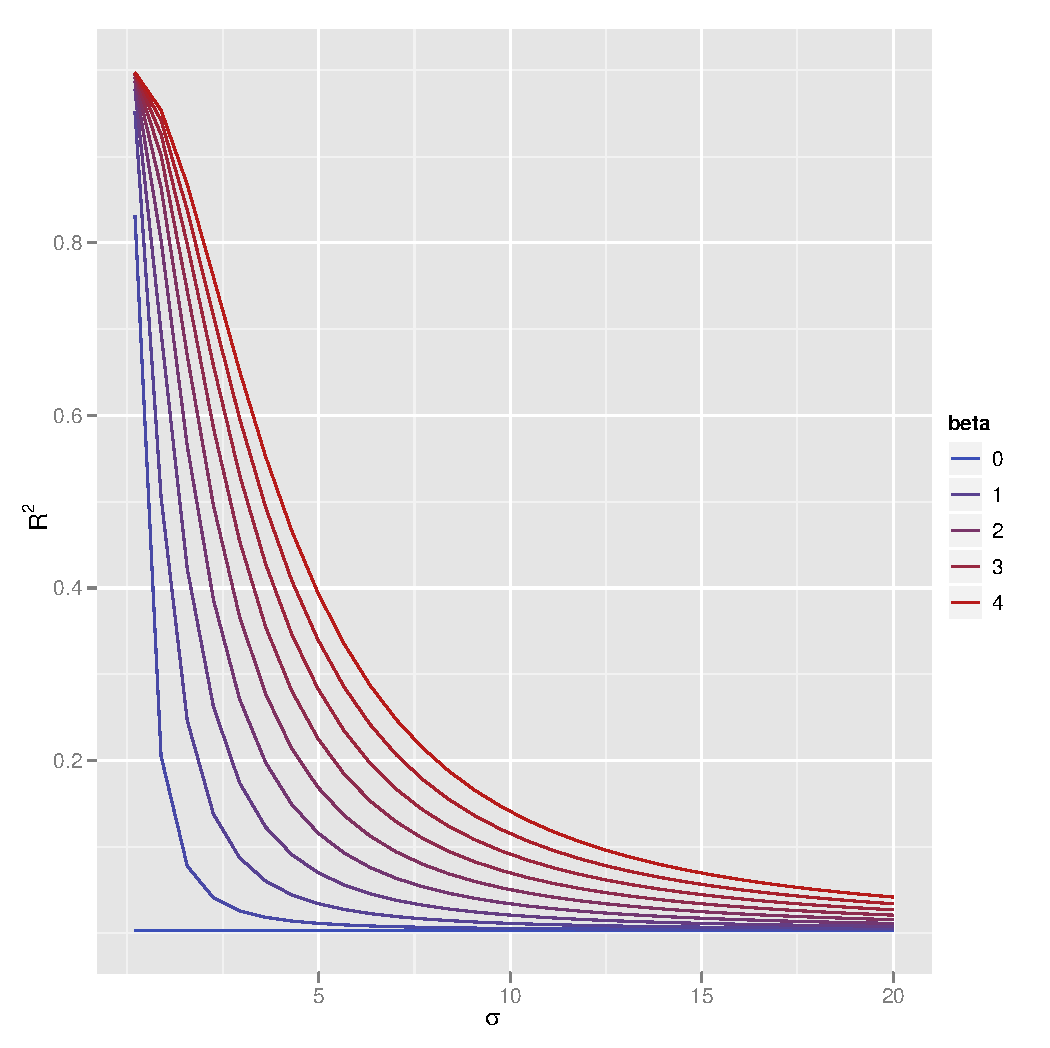
\includegraphics{rsquare_beta_sigma_lines1.pdf}}       
%       \caption{Relationship of $R^2$ with $\sigma$ and $\beta$ for sample size $n =300$. The values for $R^2$ goes down sharply with $\sigma$ and $\beta$.}
%       \label{fig:rsq}
%\end{figure}
%



%\bibliographystyle{plain}
\bibliographystyle{asa}
\bibliography{references} 


\end{document}


